% Preserve the accepted raster panels; replace only visible legends and approved titles.
% Coordinates use each source image's native 900-pixel width and top origin.
\newcommand{\vaeTrainingPanels}[1]{%
    \begingroup
    \definecolor{vaeLegendBackground}{HTML}{F8FAFC}%
    \definecolor{vaeLegendInk}{HTML}{0F172A}%
    \ifcase#1\def\vaePanelHeight{794}%
    \or\def\vaePanelHeight{854}%
    \or\def\vaePanelHeight{774}%
    \fi
    \newcommand{\vaeLegend}[3]{%
        \fill[vaeLegendBackground]
            ({##1/900},{1-(##2-9)/\vaePanelHeight}) rectangle
            ({(##1+132)/900},{1-(##2+9)/\vaePanelHeight});
        \node[anchor=west,font=\sffamily\fontsize{6.4}{7.4}\selectfont,
            text=vaeLegendInk] at ({##1/900},{1-##2/\vaePanelHeight}) {##3};}%
    \newcommand{\vaeTitle}[4]{%
        \fill[vaeLegendBackground]
            ({(##1-5)/900},{1-(##2-17)/\vaePanelHeight}) rectangle
            ({880/900},{1-(##2+17)/\vaePanelHeight});
        \node[anchor=west,font=\sffamily\bfseries\fontsize{##3}{##3}\selectfont,
            text=vaeLegendInk] at ({##1/900},{1-##2/\vaePanelHeight}) {##4};}%
    \begin{tikzpicture}[inner sep=0pt,outer sep=0pt,baseline=(panel.south)]
        \node[anchor=south west] (panel) at (0,0) {%
            \ifcase#1%
                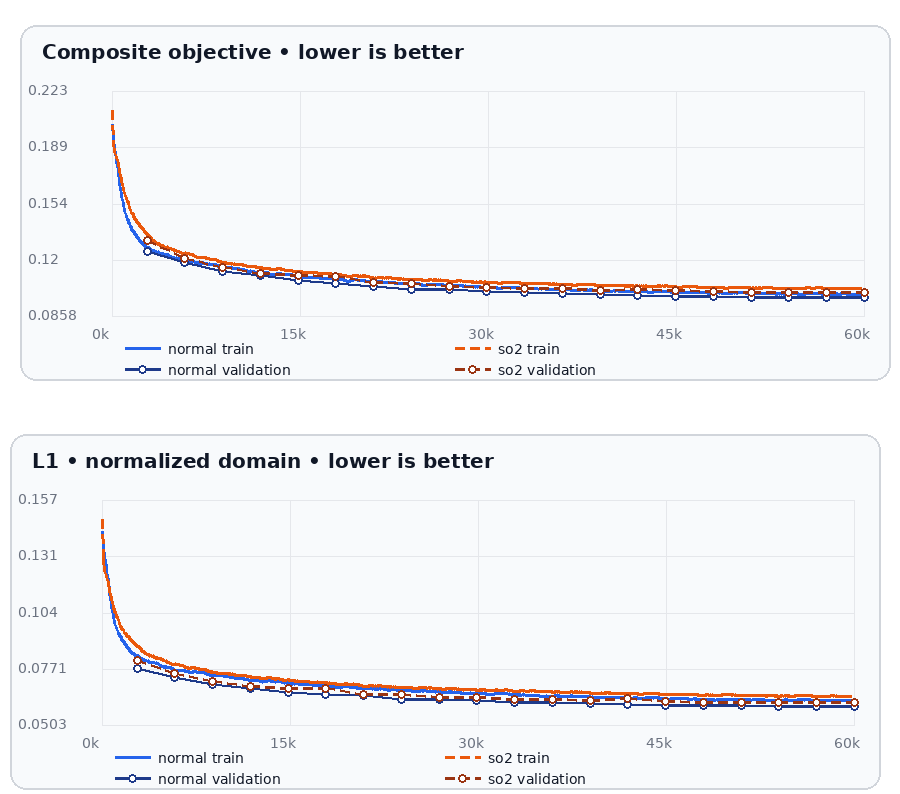
\includegraphics[width=0.88\textwidth]{vae_training_loss_panels.png}%
            \or
                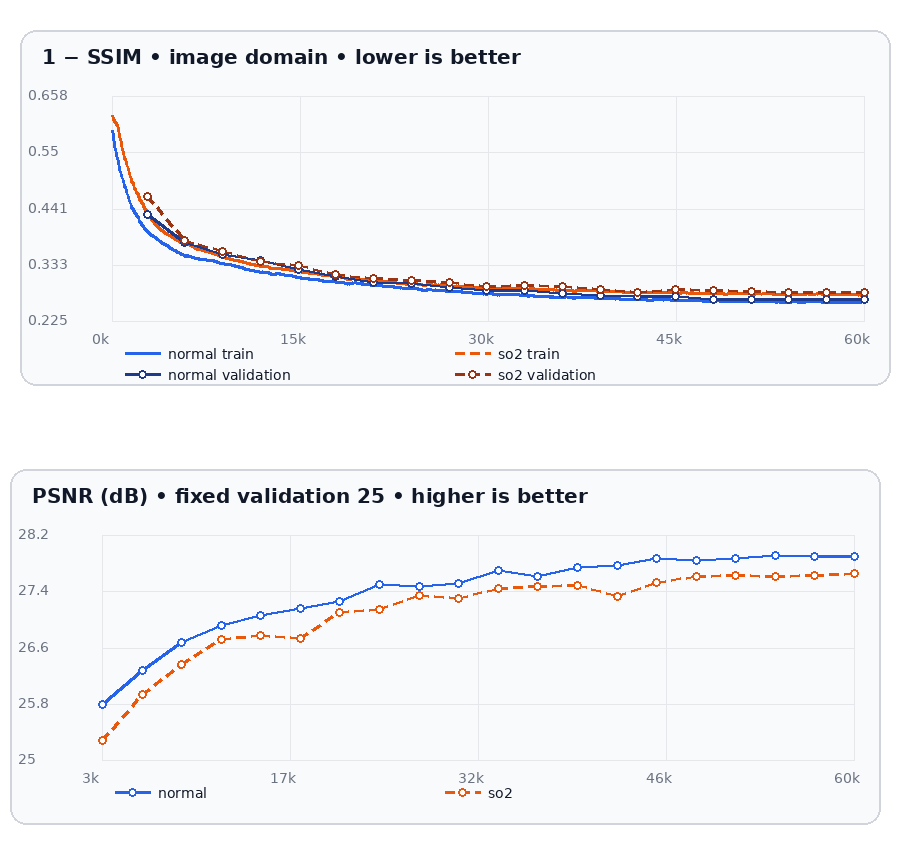
\includegraphics[width=0.88\textwidth]{vae_training_quality_panels.png}%
            \or
                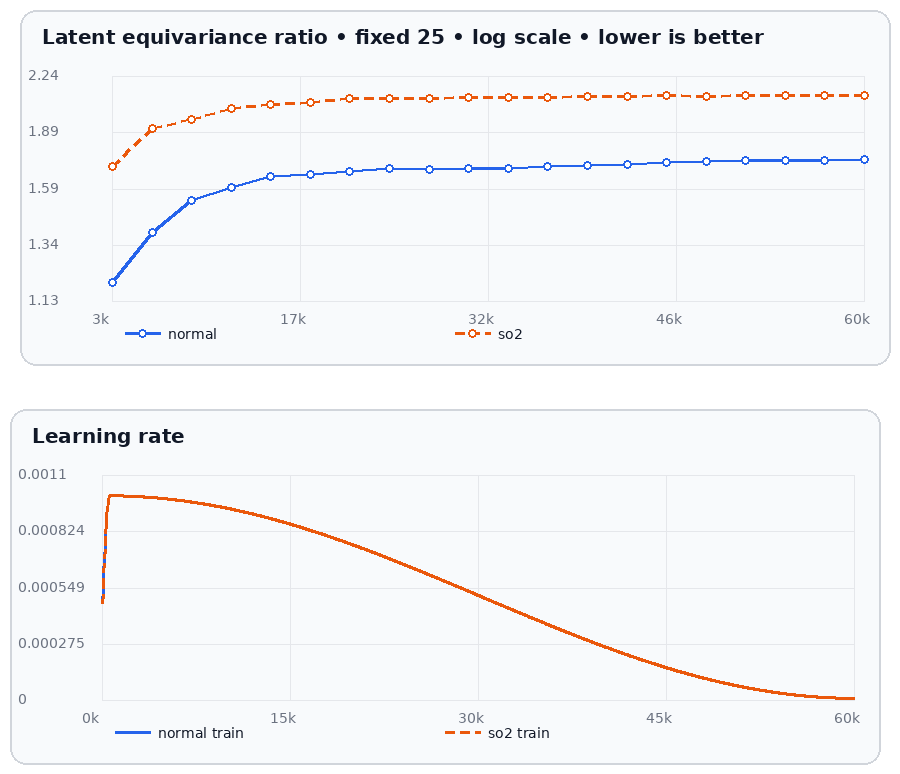
\includegraphics[width=0.88\textwidth]{vae_training_control_panels.png}%
            \fi};
        \begin{scope}[x={(panel.south east)},y={(panel.north west)}]
            \ifcase#1
                \vaeTitle{42}{53}{9.2}{Objetivo compuesto \textbullet{} menor es mejor}
                \vaeTitle{32}{463}{9.2}{MAE \textbullet{} dominio normalizado \textbullet{} menor es mejor}
                \vaeLegend{167}{348}{VAE base: entrenamiento}
                \vaeLegend{498}{348}{VAE-SO(2): entrenamiento}
                \vaeLegend{167}{370}{VAE base: validación}
                \vaeLegend{498}{370}{VAE-SO(2): validación}
                \vaeLegend{157}{758}{VAE base: entrenamiento}
                \vaeLegend{488}{758}{VAE-SO(2): entrenamiento}
                \vaeLegend{157}{779}{VAE base: validación}
                \vaeLegend{488}{779}{VAE-SO(2): validación}
            \or
                \vaeTitle{42}{58}{9.2}{\(1-\mathrm{SSIM}\) \textbullet{} dominio de imagen \textbullet{} menor es mejor}
                \vaeTitle{32}{498}{9.2}{PSNR (dB) \textbullet{} validación fija: 25 parches \textbullet{} mayor es mejor}
                \vaeLegend{167}{354}{VAE base: entrenamiento}
                \vaeLegend{498}{354}{VAE-SO(2): entrenamiento}
                \vaeLegend{167}{375}{VAE base: validación}
                \vaeLegend{498}{375}{VAE-SO(2): validación}
                \vaeLegend{157}{793}{VAE base}
                \vaeLegend{488}{793}{VAE-SO(2)}
            \or
                \vaeTitle{42}{38}{8.4}{Razón de equivarianza latente \textbullet{} 25 parches fijos \textbullet{} escala logarítmica \textbullet{} menor es mejor}
                \vaeLegend{167}{334}{VAE base}
                \vaeLegend{498}{334}{VAE-SO(2)}
                \vaeLegend{157}{734}{VAE base: entrenamiento}
                \vaeLegend{488}{734}{VAE-SO(2): entrenamiento}
            \fi
        \end{scope}
    \end{tikzpicture}%
    \endgroup}
